Validation of Napali hinges on the validation of performance of the OPQ Boxes. Some of the detection capability of the OPQ Boxes has already been characterized as shown in the previous section, however transient response and the $V_{rms}$ response are yet to be confirmed. Once the OPQ Box sensitivity has been characterized, the detection capability of Makai system must be crosschecked. First synthetic triggering streams will be injected into Makai. Next the full system will be deployed at the University of Hawaii Manoa for in-situ validation.

\section{OPQ Box Validation.}
So far only the frequency sensitivity of the OPQ Box has been validated empirically. The transient and as well as $V_{rms}$ response characterization will first be performed using synthetic data. Robust methods for generating power quality events are present in literature, and thus no new research for single device validation is required.\cite{kumar2015power}\cite{tan2013simulation} Next once the DSP software is characterized, synthetic PQ data will be loaded into a SDG1025 signal generator, and fed into the OPQ Box hardware. Any discrepancy between the DSP, and hardware-in-the-loop characterization will be noted and analyzed. The main characteristics to be validated are as follows:
\begin{itemize}
  \item{DC response:} Accuracy of the OPQ Box in measurement of a DC voltage.
  \item{$V_{rms}$ response:} Accuracy of the OPQ Box in measurement of a small changes in the amplitude of AC waveform.
  \item{THD response:} Accuracy of the OPQ Box in measurements of small harmonics mixed with a large fundamental AC waveform.
  \item{Transient response:} Validating the response of the OPQ Box metrics to various transients.
\end{itemize} 
These tests will provide a baseline for the detection capabilities of the Napali system, and result in a publication regarding the OPQ Box detection capabilities.

\section{Napali Validation.}
In order to validate OPQ system as a whole it will be deployed across the University of Hawaii Manoa campus(UH). This location is ideal because it is a relatively isolated microgrid connected to the Oahu powergrid only via a single 46kV feeder as shown in figure \ref{expdes:fig:1}. Another advantage of the UH campus is the high number of smart meters deployed, across various levels of the power delivery infrastructure. While these meters are mainly geared towards monitoring power consumption they do have some power quality monitoring capabilities. Data provided from these meters can be used in two distinct applications. First of all, this data can be used to pinpoint the section of the University of Hawaii power grid which experience a higher likelihood of power quality disturbances. These portions of the grid will have a higher spacial density of OPQ Boxes. Secondly, data from the campus deployed meters can be used as ground truth for comparison against the measurements, and analysis performed by the OPQ project. The location of smart meters in the grid topology is shown in figure \ref{expdes:fig:1} as the $M$ nodes. As evident by the meter location none of them are monitoring the consumer level power and mainly focus on the higher voltage power delivery. This placement is evidenced from the smart meter role as a consumption monitor, and thus the deployment of the OPQ Boxes at the residential level will compliment the current power quality monitoring capabilities without introducing redundancies. Finally University of Hawaii powergrid is supplying a highly diverse infrastructure. Beyond the traditional residential equipment such as computers and consumer grade electronics, UH power grid powers scientific and laboratory equipment, machine shops, and server farms. All of these elements have varying requirements/tolerances for power quality anomalies as well as different levels of power quality "pollution". Furthermore some of the electricity consumers in the UH campus is entirely unique. For example the free electron laser located in the Watanabe Hall is one of the only free electron lasers in the world, and the impact/sensitivity of power quality on the instrument are completely unstudied.
\begin{figure}[h]
	\centering
	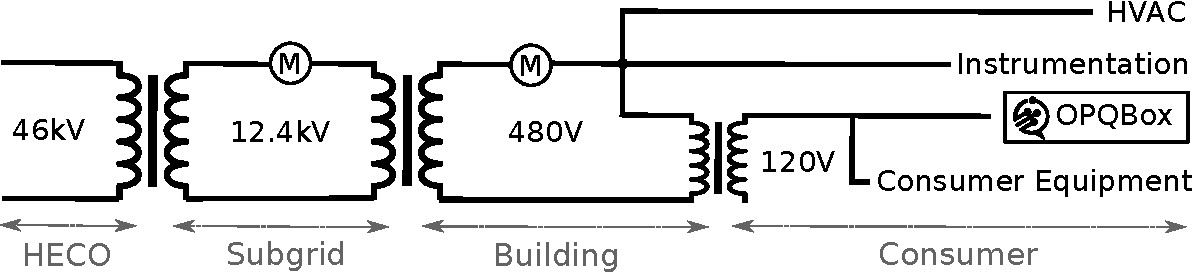
\includegraphics[width=1\linewidth]{img/uh-grid.pdf}	
	\caption{University of Hawaii at Manoa power delivery infrastructure.}
	\label{expdes:fig:1}
\end{figure}
Open power quality project acquired cloud infrastructure from the the Information Technology Services of University of Hawaii which is hosted on the Manoa campus. This allows for low latency operation, and keeps all of the traffic constrained to the UH internal network. Furthermore UH hosts a Stratum 1 NTP server. This provides UH OPQ deployment with a low latency, high precision time keeping option. Finally, OPQ project received the Presidents Green Initiative Award in spring 2018. Besides a \$10,000 monetary award, this provides the OPQ project with access to all of the buildings on campus, expertise of the engineers who oversee the campus power infrastructure, as well as access to all of the smart meter measurements already deployed across the University. 

There are 74 smart meters deployed across the UH campus. These meters measure the fundamental frequency $V_{rms}$, power consumption, reactive power, and power factor. Data from these meters will be cross-referenced with the Napali detection system in order to ascertain it's benefits. Validations of the benefits of the Napali framework will follow the framework described in Section \ref{intro:sec:claim}. Here we examine the analysis required to complete each claim in detail.

\subsection{Napali Bandwidth usage} \label{iexp:sec:band}
In order to analytically compute the bandwidth savings of the Napali compared to a system which sends all the data to the sink I will keep track of the amount of bandwidth Napali monitoring system consumed during its deployment on UH campus. This will in turn be compared to the bandwidth required by the OPQ Boxes if they were sending the entirety of the data to the sink, and establish the bandwidth efficiency of the Napali framework. In order to monitor the bandwidth of the system in-situ, an iptables bandwidth accounting will be enabled on the sink node. With the accounting enabled, I will be able to extract the exact amount of bytes transfered by the Napali framework during the deployment period. Since the sampling rate of the OPQ Box is well characterized, and the number of OPQ Boxes is fixed it is trivial to calculate the amount of raw data generated by the OPQ network during any time period. In order to make this comparison fair, the raw data bandwidth will be scaled by the compression ratio of the state of the art compression algorithm specifically designed for power quality measurements.\cite{zhang2009new}

\subsection{Sink processing requirement under the Napali Framework} \label{iexp:sec:scale}
In order to evaluate the scalability of the sink node under the Napali framework, synthetic data containing a small amount of distributed events will be injected into the Makai triggering system. While the synthetic data for a single point PQ disturbance is easily generated, distributed PQ event generation is not well developed. However there is some literature concerning power fault propagation and localization. \cite{parsons1998direction} \cite{polajvzer2017evaluation} The main takeaway from these authors is the energy and amplitude of the event diminishes with electrical distance from the source. As such, by generating a single point PQ event as described in \cite{kumar2015power}\cite{tan2013simulation}, and linearly scaling it based on the simulated electrical distance from the source, a distributed PQ event ensemble can be generated. These events will be ran through the simulated OPQ Box DSP stack and the extracted metrics will be propagated to the Makai aggregation sink. The number of simulated OPQ Box devices that can be supported on a single node will be recorded, and will provide the baseline for the Makai sink node capabilities. Next, the same dataset will be processed on the same node using simulated OPQ Box software stacks. The amount of concurrent processes which are able to keep up with the targeted sampling rate of $12kS/s$ will be determined and recorded, and compared to the amount of devices which can be supported by Makai.

\subsection{Effects of latency in the Napali framework} \label{iexp:sec:lat}
Latency of Napali triggering system has significant impact on its ability to read out complete raw data events. Using generated distributed events as a baseline, I will be able to tune the threshold and temporal requirements for Makai detection algorithms. Furthermore, temporal, spacial, and amplitude noise will be injected into the generated datasets, to simulate various uncertainties with regards to data collection, such as local noise, and NTP offset errors. Taking into the account the detection latency of Makai, if some of the requested data is no longer available on the OPQ Box, only a partial time window will be returned. These events will be marked as incomplete and their fraction as compared to the total number of events recorded will be used to establish the latency tolerance of the Napali framework. 
Synthetic benchmarks will be carried out to establish the latency that the Napali system can incur without losing a portion of the event. Since this is highly dependent on the amount of storage allocated for the RDRB, these experiments will be carried out with various RDRB settings.

\subsection{Temporal Locality triggering of the Napali framework} \label{iexp:sec:loc}
Once the OPQ Box is fully validated and the Makai detection thresholds are tuned using synthetic datasets, the Napali system will be fully deployed at the University of Hawaii at Manoa.  Every time the Napali detects an event, both OPQ Boxes and building meters will be queried for data. While it may be unfeasible to query raw data from the UH metering infrastructure, metrics are readily available. This data will be used to ascertain the proportion of false positive events detected by Napali. Additionally, the internal single point fault detection mechanism of the UH power meters will be used in conjunction with the events detected by Napali to measure the rate of false negative events. Both the false negative and false positive measurements will be used to ascertain the detection efficient of the Napali framework. This analysis will also include an evaluation  of Napali`s ability to reject single point anomalies. For a portion of OPQ deployment, every event triggered by a single device will be captured. These events will be analyzed in order to determine if a gridwide anomaly was incorrectly classified as a single point disturbance. 

\subsection{Sub-threshold Data Acquisition} \label{iexp:sec:sub}
Napali methodology will be compared with the single point anomaly detection. In order to do that I will compare the extent to which the sub-threshold portion of events are missed by the UH metering infrastructure. In a large distributed event, if a portion of events is not detected by the UH meter`s single point detection, but picked up by the Napali framework, these events will be flagged and analyzed for their merit. This will in turn provide a metric of distributed detection ability of the Napali framework compared to the commercial system. Furthermore, for a portion of the deployment the triggering stream from the OPQ Boxes will be stored along with the acquired raw data. The triggering stream can be used to compute which fraction of devices would have self triggered if operating autonomously. This will provide the baseline for sub-threshold triggering efficiency of the Napali system, with respect to the single point detection ability of the OPQ Box.

\section{Napali Framework in Other Domains}
The work outlined above will allow me to characterize the benefits and drawbacks of the Napali architecture. Armed with this knowledge I intend to examine the examine the possibility of using a similar architecture in other domains. Napali approach could prove useful in general sensor network design, as well as IOT and other domains which rely on anomaly detection. This contribution will involve an additional literature review of anomaly detection systems, and proposals to integrate Napali-like methodology to improve their efficiency and reduce their bandwidth consumptions.


\section{Schedule}
Bellow is the time-line describing the major research activities leading up to my defense.

\begin{center}
\begin{tabular}{ ||c | c c|| }
\hline
 \textbf{Activity} & \textbf{Start Date} & \textbf{End Date} \\ 
 \hline
 \hline
 OPQ Box 2 Validation & October 1\textsuperscript{st} & November 31\textsuperscript{st} \\  
 Makai Validation & October 15 1\textsuperscript{st} & November 30\textsuperscript{th}   \\
 Data Collection & December 1\textsuperscript{st} & TBD   \\
 OPQ Box 2 Instrumentation paper & January 1\textsuperscript{st} & February 1\textsuperscript{st}   \\
 Data Analysis & February 1\textsuperscript{st} & March 1\textsuperscript{st}  \\
 Introduction Dissertation Chapter & March 1\textsuperscript{st}  & March 15\textsuperscript{th}  \\
 Literature Review Dissertation Chapter & March 15\textsuperscript{th} & April 1\textsuperscript{st}  \\
 Experimental Design Dissertation Chapter & April 1\textsuperscript{st} & April 15\textsuperscript{th}  \\
 Analysis Dissertation Chapter & April 15\textsuperscript{th} & May 15\textsuperscript{th}  \\
 Conclusions Dissertation Chapter & May 15\textsuperscript{th} & June 15\textsuperscript{th}  \\
 \hline
 
\end{tabular}
\end{center}
